\subsection{Mengder}
\begin{frame}{Sett / Mengder}
    Et sett, eller en mengde, er en slags liste av objekter, bortsett fra:\\
    \indent \hspace{3mm}    1. Det inneholder ingen duplikater\\
    \indent \hspace{3mm}    2. Det har ingen konkret rekkefølge
    
    \pause
    \begin{block}{Eksempel}
        Alle de følgende settene er like: \\
        $\{1, 2, 3\}$, $\{3, 2, 1\}$ \\
        $\{1, 1, 1, 1, 2, 2, 3, 3\}$
    \end{block}
    
    \pause
    \begin{block}{Eksempel}
        $1 \in \{1, 2, 3\}$ = T \\
        $5 \in \{1, 2, 3\}$ = F
    \end{block}
\end{frame}


\begin{frame}{Kjente sett}
    Flere sett bruker vi veldig ofte. Her er noen av dem.\\
    
    \begin{tabular}{c|l|c}
        Symbol & Navn & Innhold \\ \hline
        $\mathbb{N}_0$ & Naturlige tall & $\{0, 1, 2, 3, ....\}$\\
        $\mathbb{Z}$ & Heltall & $\{... -2, -1, 0, 1, 2, 3, ....\}$\\
        $\mathbb{Q}$ & Rasjonale tall & $\{-3/2, 1/10, 4/5, 5/4, ....\}$\\
        $\mathbb{R}$ & Reelle tall & $\{\pi, e, 0.111111111..., 2\pi, .....\}$\\
        $\emptyset$ & Det tomme settet & $\{\}$
    \end{tabular}
    
\end{frame}

\begin{frame}[fragile]{Settbyggingsnotasjon}
    Istedet for å manuelt skrive opp alle elementene i et sett, eller å bruke uformell \enquote{...}-notasjon, kan vi bruke setbyggingsnotasjon.
    \begin{block}{Eksempler}
        $\{ x | x \in \mathbb{N}\}$ = $\mathbb{N}$\\
        $\{ x \cdot 2 | x \in \mathbb{N}\}$ = $\{0, 2, 4, 6, 8, ....\}$\\
        $\{x | x \in \mathbb{N}, x$ mod $3 = 0 \} = \{0, 3, 6, 9, ...\}$\\
        $\{x/2 | x \in \mathbb{N}, x$ mod $3 = 0\} = \{0, 1.5, 3, 4.5, ...\}$
    \end{block}
    \pause
    \begin{python}
[ x for x in range(100) ]
[ x*2 for x in range(100) ]
[ x for x in range(100) if x % 3 == 0 ]
[ x/2 for x in range(100) if x % 3 == 0 ]
    \end{python}
\end{frame} 

\begin{frame}{$\cup$, $\cap$, $\bar{}$ og $-$}
    $A \cup B := \{x | x \in A \lor x \in B\}$ \\
    $A \cap B := \{x | x \in A \land x \in B\}$\\
    $A - B = A \backslash B := \{x | x \in A\land  x \notin B\}$\\
    $A^C = \bar{A} := \{x | x \notin A\}$
    
    \begin{figure}%
        \centering
        \subfloat[\centering $A \cup B$]{{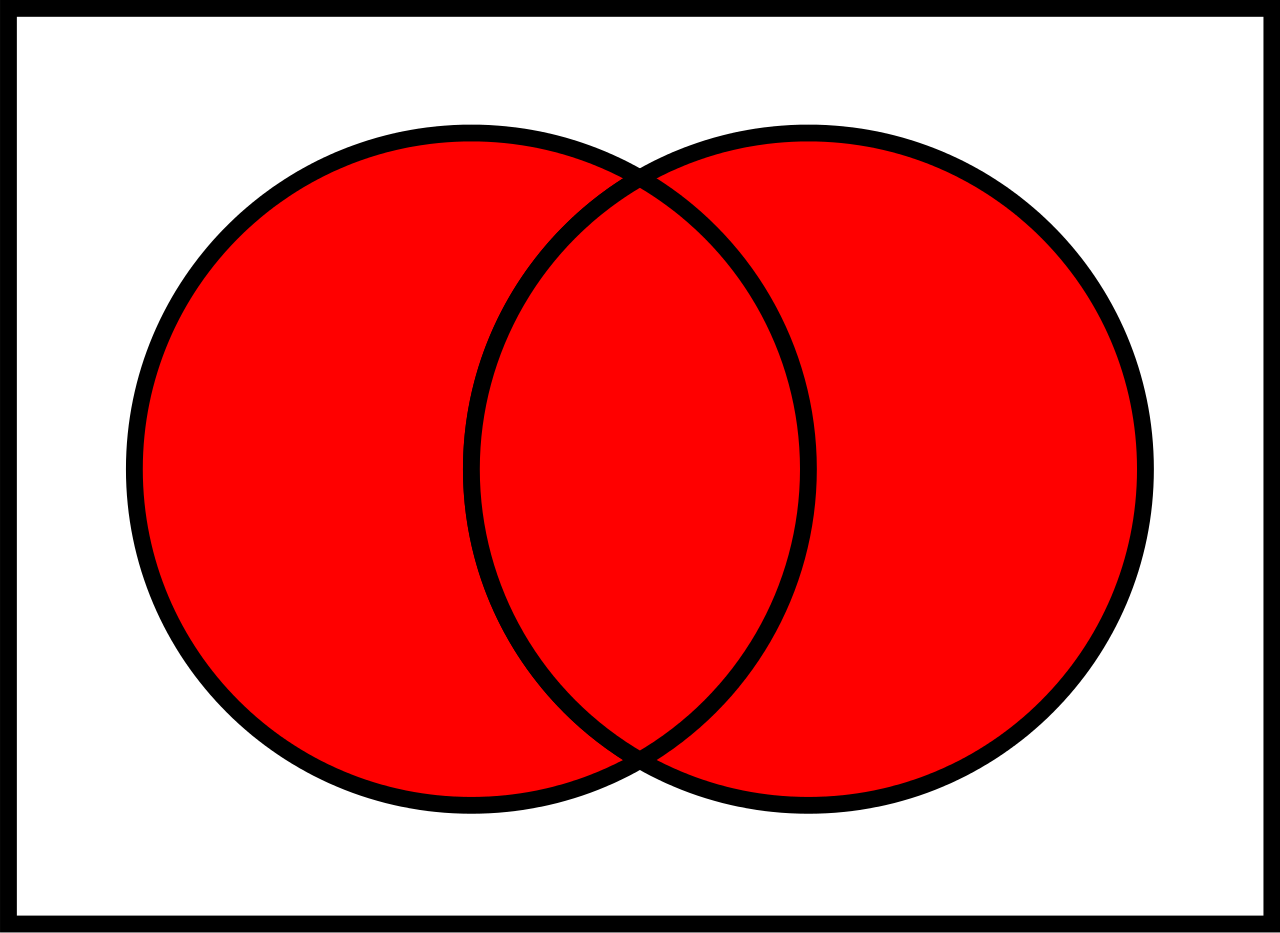
\includegraphics[width=2.5cm]{images/union.png} }}%
        \qquad
        \subfloat[\centering $A \cap B$]{{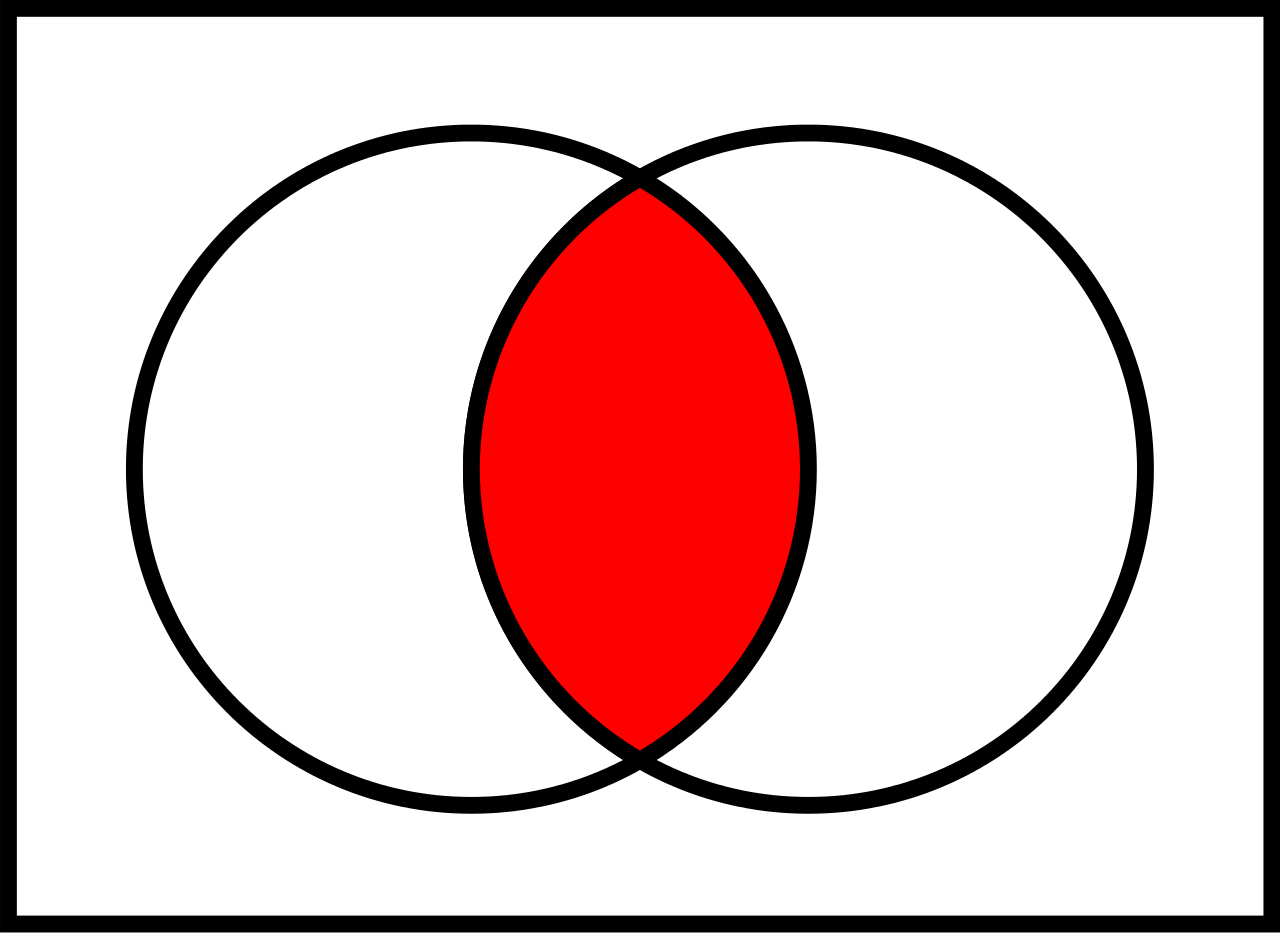
\includegraphics[width=2.5cm]{images/snitt.png} }}%
        \qquad
        \subfloat[\centering $B - A$]{{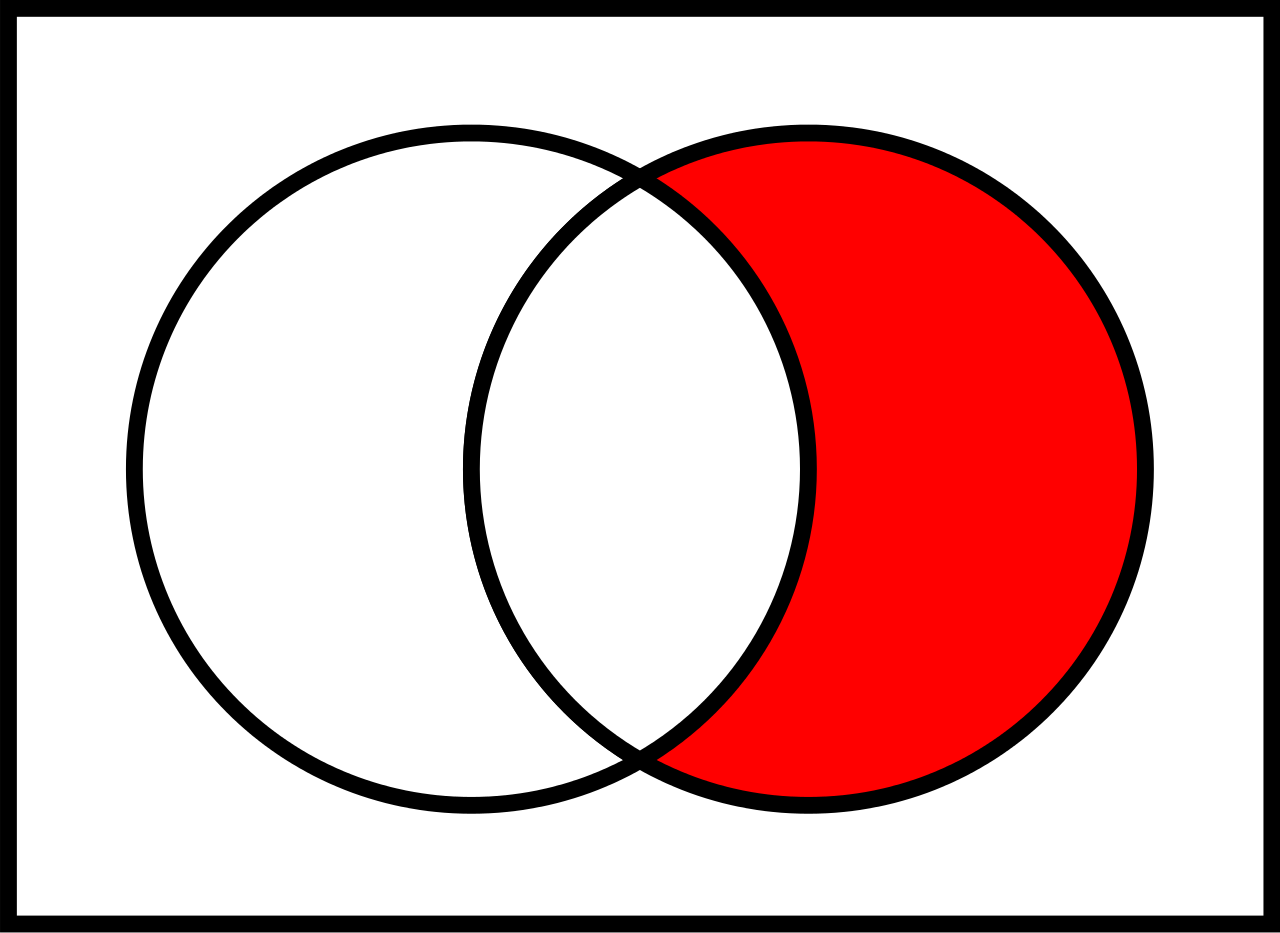
\includegraphics[width=2.5cm]{images/minus.png} }}%
        \qquad
        \subfloat[\centering $\bar{A}$]{{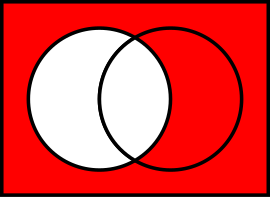
\includegraphics[width=2.5cm]{images/complement.png} }}%
        % \caption{Vennediagramer}%
        \label{fig:example2}%
    \end{figure}
\end{frame}

\begin{frame}{$\subset, \subseteq, =, \supseteq, \supset$}
    Vi har flere måter å uttrykke at et sett inneholder elementer fra et annet sett.
    \begin{itemize}
        \item $A \subseteq B := \forall x \in A : (x \in B)$
        %\item $A \supseteq B := B \subseteq A$
        \item $A \subset B := A \subseteq B \land \exists x \in B : (x \notin A)$
        %\item $A \supset B := B \subset A$
        \item $A = B := A \subseteq B \land B \subseteq A$
    \end{itemize}
    \pause
    \begin{block}{Eksempler}
        $\{1\} \subseteq \{1, 2\}$ = T\\
        $\{1\} \subseteq \{5\}$ = F\\
        $\{a, b\} \subset \{a, b\}$ = F\\
        $\{a, b\} \subseteq \{a, b\}$ = T
    \end{block}
    \pause
    \centering
    Obs! Enkelte skriver $\subset$ når de mener $\subseteq$, og $\subsetneq$ når de mener $\subset$.
\end{frame}

\begin{frame}{Tavleoppgaver fra H19}
    \begin{itemize}
        \item Vis eller motbevis at $(A - C) \cap (B - C) = \emptyset.$
        \item Vis eller motbevis at $(A - C) \cap (C - B) = \emptyset.$
    \end{itemize}
    
    For å løse det med vennediagrammer:
    \begin{enumerate}
        \item Tegn et vennediagram. Begynn med sirkler for A, B, etc.
        \item Fargelegg områdene til deluttrykkene, dvs $(A - C)$ og $(B - C)$ i dette eksemplet.
        \item Bruk områdene i deluttrykkene til å farge omårdene i de større uttrykkene, dvs hele $(A - C) \cap (B - C)$ her.
        \item Er områdene til hele uttrykkene på hver side av = det samme?
    \end{enumerate}
    \pause
    Alternativt: bruk definisjonene til $\cap$, $\cup$, etc til å omformulere uttrykket.
\end{frame}

\begin{frame}{Nyttige regler for sett}
        \begin{tabular}{l|c}
        Ekvivalens & Navn \\ \hline
        $A \cap U = A$ & Identity\\
        $A \cup \emptyset = A$ \\ \hline
        
        $A \cup U = U$ & Domination\\
        $A \cap \emptyset = \emptyset$\\ \hline
        
        $A \cup A = A$ & Idempotent\\
        $A \cap A = A$ \\ \hline
        
        $A = (A^C)^C$ & Negation\\ \hline
        
        $A \cup B = B \cup A$ & Commutative\\
        $A \cap B = B \cap A$ \\

    \end{tabular}
    \hfill
        \begin{tabular}{l|c}
        Ekvivalens & Navn \\ \hline
        
        $(A \cup B) \cup C = A \cup (B \cup C)$ & Associative\\
        $(A \cap B) \cap C = A \cap (B \cap C)$ \\ \hline
        
        $A \cup (B \cap C) = (A \cup B) \cap (A \cup C)$ & Distributive\\
        $A \cap (B \cup C) = (A \cap B) \cup (A \cap C)$ \\ \hline
        
        $(A \cap B)^C = A^C \cup B^C$ & De Morgan \\
        $(A \cup B)^C = A^C \cap B^C$ \\ \hline
        
        $A \cup (A \cap B) = A$ & Absorption \\
        $A \cap (A \cup B) = A$ \\ \hline
        
        $A \cup A^C = U$ & Negation \\
        $A \cap A^C = \emptyset$ \\
        \end{tabular}
\end{frame}

\begin{frame}{Kardinalitet}
    Om $A$ er et sett, er $|A|$ antall elementer i settet, \textit{kardinaliteten}, eller \textit{lengden}.\\
    To sett har samme kardinalitet om de har samme lengde.
    \begin{block}{Eksempler}
        $|\{a, b, c\}| = 3$ \\
        $|\{\}| = |\emptyset| = 0$\\
        $|\mathbb{N}| = \aleph_0$
    \end{block}
\end{frame}